\label{sec:relatedworks}
\subsection{Генеративные состязательные сети}

Генеративные состязательные сети (\emph{Generative adversarial network}, сокр., \emph{GAN})  это семейство генеративных моделей, разработанное Яном Гудфеллоу в 2014 году \cite{goodfellow2014generative}.  Они формулируют процесс ~обучения (подгонки, fitting) генеративной модели~ в виде антагонистической игры между двумя игроками: \emph{генератором} и \emph{дискриминатором}.

% набор синтетических данных. Эти данные represent выучиваемое распределение q(x) 
% пытаясь аппроксимировать обучающую выборку, полученную из распределения реальных данных $q_{data}(x)$
Генератор $G$ представляет собой глубокую нейронную сеть, задающую отбражение из латентного пространства $Z$ в пространство данных $\mathcal X$.
Принимая на вход случайные вектора из некоторого заданного распределения $p(z)$ в $Z$, он производит набор синтетических данных, пытаясь аппроксимировать распределение обучающей выборки $q_{data}(x)$.

% распределения реальных данных $q_{data}(x)$ ?== распределение обучающей выборки $q_{data}(x)$
Дискриминатор $D$ представляет собой глубокую нейронную сеть, задающую отбражение из пространства данных $\mathcal X$ в $\mathbb R$. Получив на вход некоторый элемент из пространства $\mathcal X$, дискриминатор ~возвращает~(характеризует) вероятность того, что он был получен из распределения реальных данных $q_{data}(x)$, а не сгенерирован генератором $G$.

\begin{figure}[h]
\begin{center}
    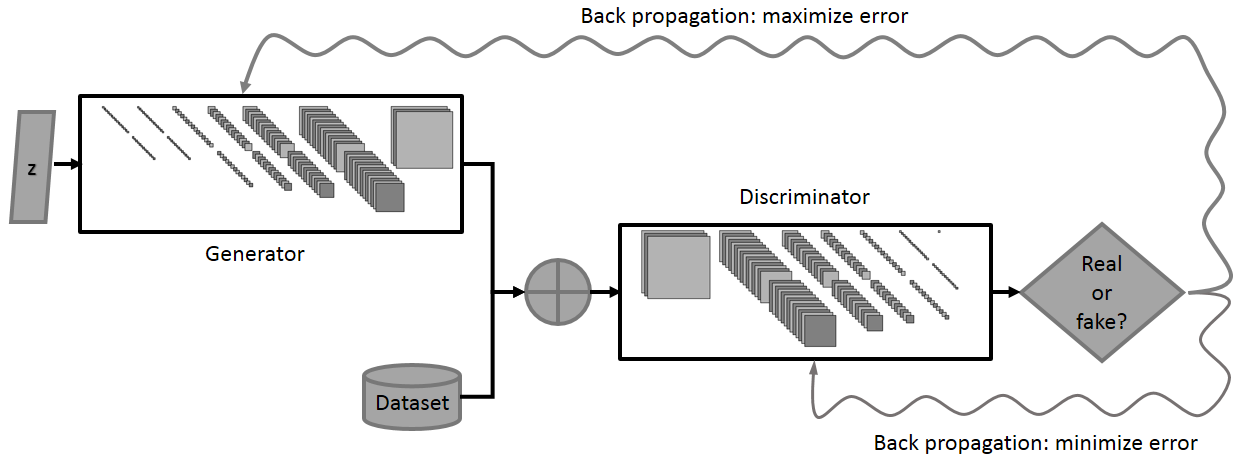
\includegraphics[width=0.9\textwidth]{gan}
    \caption{Архитектура генеративной состязательной сети (написать откуда взял)}
    \label{fig:subim11}
\end{center}
\end{figure}

Роль дискриминатора состоит в том, чтобы как можно более точно отличать синтетические данные, полученные генератором, от реальных данный, взятых из обучающей выборки, в то время как генератор пытается обмануть дискриминатор путем генерирования синтетических данных, как можно более похожих на реальные.
% Following the more general formulation introduced in [39], the GAN learning problem entails finding the minimax with respect to the pair(G,D) (i.e., the Nash equilibrium), of the value function defined as
Процесс совместного конкурентного обучения продолжается вплоть до достижения парой $(G, D)$ <<седловой точки>> (т.е. равновесия по Нэшу) \cite{goodfellow2017nips} функции выигрыша
$$
\min_{G} \max_{D} V(G, D) = \mathop{\mathbb{E}}_{x \sim q_{data}(x)} [\log D(x)] + \mathop{\mathbb{E}}_{z \sim p(z)} [\log (1 - D(G(z)))] ,
$$
в которой генератор способен генерировать данные, неотличимые дискриминатором от реальных.

%Since the generator (decoder) is a composition of linear maps and activation functions, its smoothness is based solely on the chosen activation functions.
%Так как и генератор, и дискриминатор являются полностью дифференцируемыми нейронными сетями, их можно совместно обучать методом обратного распространения ошибки, используя одну функцию потерь.

\subsection{Генеративные нейронные сети для генерации лиц}

% Нужно тут водинисто вводить в задачу генерации изображений, не перечислять решения, а рассказывать как кокой-то таймлаин.

Ряд специализированных особенностей в задаче генерации изображений (в.т.ч. изображений лиц).
Дискриминатор предстваляет собой сверточную нейронную сеть [VGG / conv ?], генератор --- сверточную нейронную сеть со слоями транспонированной свертки [DCGAN].
Пространство данных $\mathcal X$ предстваляет собой пространство изображений, каждый элемент которого обладает некоторым набором семантических признаков, в случае лиц, пол или возраст.
%Тут нужно сказать про латентное пространство, и рас уж мы заговорили про семантические признаки, то curvature и disentanglement.

% можно выкинуть пункты и рассказывать в одном нарративе (особенно если будет какое-то сравнение).

\subsubsection{BigGAN}
% ... разработанная компанией DeepMind.
BigGAN \cite{bigGAN} – это генеративная состязательная сеть, спроектированная с целью масштабирования архитектуры для генерации изображений высокого разрешения.
% Че то про увеличение кол-ва параметров(весов) в 2 раза

% ! Это не имеет особого отношения к теме работы, поэтому не надо !
% https://machinelearningmastery.com/a-gentle-introduction-to-the-biggan/
% https://arxiv.org/abs/1805.08318  таких как self-attention слой
% https://arxiv.org/abs/1802.05957  спектральная нормализация весов
Она вносит ряд модификаций в стандартную архитектуру генеративных состязательных сетей, что позволяет добиться качественной генерации изображений с разрешением до $512\times512$ на самых разнообразных классах изображений.


% Если пункты будут выкинуты (и будет сравнение) то стоит перенести это за StyleGAN.
\subsubsection{ALAE}
%https://arxiv.org/pdf/1511.05644.pdf  Adversarial Autoencoders
%We designed an AE architecture where we allow the latent distribution to be learned from data to address entanglement (A). The output data distribution is learned with an adversarial strategy (B). Finally, to implement (A) and (B) we impose the AE reciprocity in the latent space (C).

% декомпозируем генератор и дискриминатор ... - но это не очень понятно
ALAE \cite{ALAE} – это генеративная нейронная сеть, которая совмещает в себе особенности генеративных состязательных сетей и вариационных автоэнкодеров [].

Она модифицирует стандартную архитектуру генеративных состязательных сетей путем добавления \emph{перед} генератором и \emph{перед} дискриминатором некоторых выучваемых отображений в промежуточное латентное пространство.
% наложение на промежуточное латентное пространство ограничения о взаимной близости представлений дает возможность выучить latent distribution с помощъю autoencoder стратегии, и data distribution с помощью состязательной стратегии.
Из-за этого он жертвует качеством генерации, но дополнительно выучивает обратное отображение в латентное пространство сети.

\subsubsection{StyleGAN}
StyleGAN \cite{StyleGAN} – это генеративная состязательная сеть, которая специализирована на генерировании реалистичных изображений лиц. 
%На момент написания работы эта сеть давала лучшие результаты в данной области.

%https://neurohive.io/ru/papers/stylegan-open-source/   
StyleGAN предлагает альтернативную архитектуру генератора, которая основывается на идеях из style transfer. Эта архитектура позволяет отделить высокоуровневые атрибуты изображения (положения лица, личность человека) от случайных вариационных факторов (волосы, веснушки и т.п.).

%Для этого генератор ...
Синтез изображения начинается с фиксированного входного вектора, а информация о латентном представлениии встраивается на каждом слое генератора.
%Our generator starts from  a  learned  constant  input  and adjusts  the  “style”  of the  image  at  each  convolution  layer  based  on  the  latent code,  therefore  directly  controlling  the  strength  of  image features at different scales.  Combined with noise injected directly into the network, this architectural change leads to automatic, unsupervised separation of high-level attributes(e.g., pose, identity) from stochastic variation (e.g., freckles,  hair)  in  the  generated  images,  and enables  intuitive scale-specific mixing and interpolation operations.  We do not  modify  the  discriminator  or  the  loss  function  in  anyway, and our work is thus orthogonal to the ongoing discussion about GAN loss functions, regularization, and hyper-parameters

% !Что нужно для работы ! :
% * маппинг из Z в W
% * стиль встраевается на каждом слое (W+)

%StyleGAN addresses the problem of curvature and disentanglement.
Одной из ключевых особенностей архитекуры StyleGAN является наличие промежуточного латентного пространства $\mathcal W$. Во время обучения StyleGAN выучивает нелинейное преобразование $f: \mathcal Z \mapsto \mathcal W$, что позволяет избавиться от ограничений, накладываемых вероятносным распределением тренировочных данных, и получить более линейное латентное пространство.

%Нужно вначале рассказать о линейности и кривизне латентного пространства и почелу это важно.
%Т.к. входное латентное пространство $\mathcal Z$ должно подстраиваться под вероятносное распределение тренировочных данных, это приводит ...
%The input latent space must follow the probability density of the training data, and we argue that this leads to some degree of unavoidable  entanglement.   Our  intermediate  latent  space is free from that restriction and is therefore allowed to be disentangled

\emph{Нужно поправить изображение и решить, насколько дословно расписывать пример}

\begin{figure}[h]
\begin{center}
    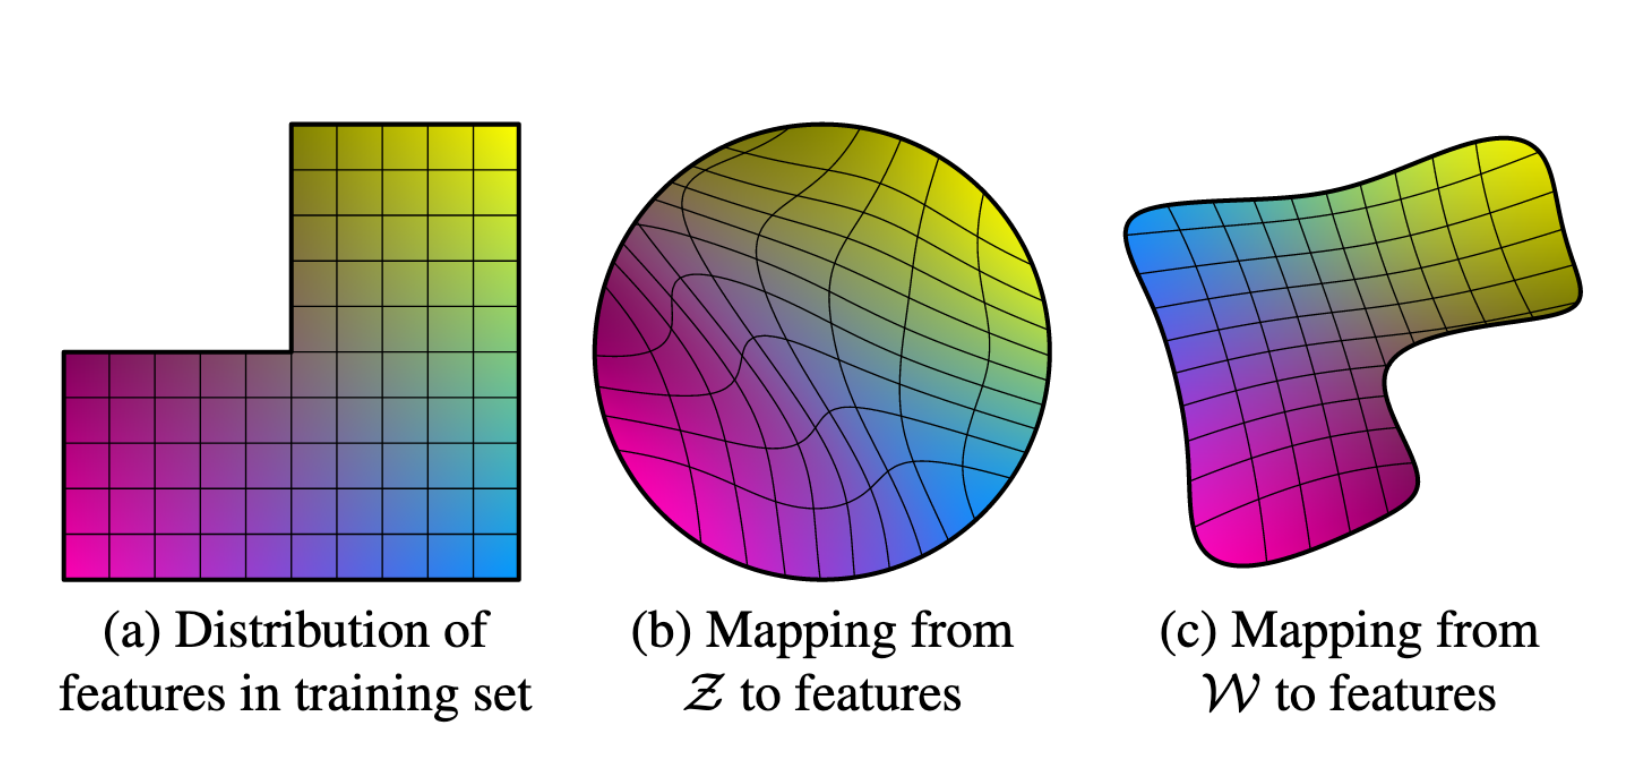
\includegraphics[width=0.7\textwidth]{stylegan_mapping}
    \caption{Иллюстрация действия промежуточного латентного пространства на примере двух факторов вариации. Изображение взято из \cite{StyleGAN}.}
    \label{fig:stylegan-mapping}
\end{center}
\end{figure}
% Illustrative example with two factors of variation (image features, e.g., masculinity and hair length).  (a) An example training set where some combination (e.g., long haired males) is missing. (b) This forces the mapping from Z to image features to become curved so that the forbidden combination disappears in Z to prevent the sampling of invalid combinations.  (c) The learned mapping from Z to W is able to “undo” much of the warping.

%Этот абзац можно выкинуть, если в эеспериментах будет сравнение bigGAN, StyleGAN (Z, W, W+)
% Иначе нужно его мотивировать, возможно написать требования
Так как при редактировании реальных фотографий точность генерации имеет критическое значение, в качестве базовой генеративной модели была взята нейронная сеть StyleGAN.

\subsection{Методы отображения реальных изображений в латентное пространство сети}

В генеративных состязательных сетях обратное отображение, позволяющее по входному изображению получить соответствующий ему латентный вектор, напрямую не задано.

\subsubsection{Обучение дополнительного энкодера}

% Здесь опять сказать про ALAE

Существующие подходы \cite{donahue2016adversarial} предлагают обучать дополнительную нейронную сеть, которая будет отображать входное изображение в латентное пространство.

\subsubsection{Латентная оптимизация}

% Здесь сказать про то что ГАН дифференциирум по входам, потому что композиция линейных и активаций.

Другие подходы \cite{perarnau2016invertible} предлагают оптимизировать латентный вектор напрямую, минимизируя некоторую функцию потерь реконструкции.

\subsection{Методы выделения семантик изображения в латентном пространстве сети}
Идея манипулирования латентным вектором в латентном пространстве генеративной состязательной сети основана на наблюдении о том, что к латентным векторам применима векторная арифметика \cite{radford2015unsupervised}.

Один из существующих подходов \cite{shen2020interfacegan} выдвигает предположение о линейности латентного пространства, и исследует его с целью нахождения векторов, соответствующих определенным заданным изменениям в признаках изображения.

Другой подход \cite{hrknen2020ganspace} использует метод главных компонент для уменьшения размерности латентного пространства и выделения наиболее важных направлений. Дальнейший качественный анализ полученных направлений показывает, что они соответствуют значимым изменениям в изображении.
